\documentclass{beamer}
\usepackage{hyperref}
\usepackage{booktabs}
\usepackage{graphicx}
\usepackage{adjustbox}
\usepackage{listings}
\usepackage{xcolor}

\lstdefinestyle{PythonStyle}{
    language=Python,
    basicstyle=\ttfamily\tiny,
    keywordstyle=\color{blue}\bfseries,
    stringstyle=\color{red},
    commentstyle=\color{green!60!black},
    morekeywords={random_state, max_iter, n_neighbors},
    frame=single,
    showstringspaces=false
}

\hypersetup{
    colorlinks=true,
    urlcolor=blue
}

\title{Pattern Recognition and Machine Learning Assignment}
\author{Ioannis Michalainas, Maria Charisi \\
    \href{https://github.com/ioannisam/PR-ML}{Github Repo}
}
\date{December 2024}

\setbeamertemplate{footline}[frame number]
\addtocounter{framenumber}{-1}

\begin{document}

\frame{\titlepage}

\begin{frame}

% PART A%

\frametitle{PART A}
In this part, our study involves the quantification of levels of stress of video game players. Our task in is to implement a Maximum Likelihood Estimator to diversify between two classes $\omega_1$ (stress) and $\omega_2$ (no stress). We need to be able to accurately classify a player based on his play-style as either stressed or not stressed (binary classification).

\end{frame}

\begin{frame}
\frametitle{Data}

To perform our analysis we use the following data 
\begin{itemize}
    \item The Probability Density Function (PDF given $\theta$)$$ p(x \mid \theta) = \frac{\pi}{1 + (x - \theta)^2} $$
    \item Training Sets $D_1$ and $D_2$ for both classes ($\omega_1$, $\omega_2$)
    \item A Discriminant Function $$ g(x) = \log P(x \mid \hat{\theta}_1) - \log P(x \mid \hat{\theta}_2) + \log P(\omega_1) - \log P(\omega_2) $$
\end{itemize}
\end{frame}

\begin{frame}
\frametitle{A1}
In this part we want to estimate variables $\theta_1$ and $\theta_2$.
We begin by implementing the log likelihood function:
$$
\log L(\theta \mid D) = \sum_{x \in D} \log p(x \mid \theta)
$$
We now need to find $\theta_1$ and $\theta_2$ that maximize this function. A first approach would be to use the gradient of $log L(\theta \mid D)$ to find the optimal $\theta$ values. However, the gradient of this function does not have a closed-form expression, making it computationally challenging to apply this method directly.
\end{frame}

\begin{frame}
\frametitle{$log L(\theta \mid D)$ maximization}
Instead, we take a simpler approach:
\begin{itemize}
    \item Define a range of candidate $\theta$ values that likely contains the true $\theta$.
    \item Evaluate the log-likelihood function for these candidates and select the $\theta$ that maximizes it.
\end{itemize}
Since the data range spans approximately [-4.5, 4.1], we select a slightly wider candidate range for $\theta$, such as [-5, 5], to ensure it includes the optimal value.
\end{frame}

\begin{frame}
\frametitle{Plot}
$\hat{\theta_1}$ estimation:  2.60
$\hat{\theta_2}$ estimation: -3.16
\begin{figure}
    \centering
    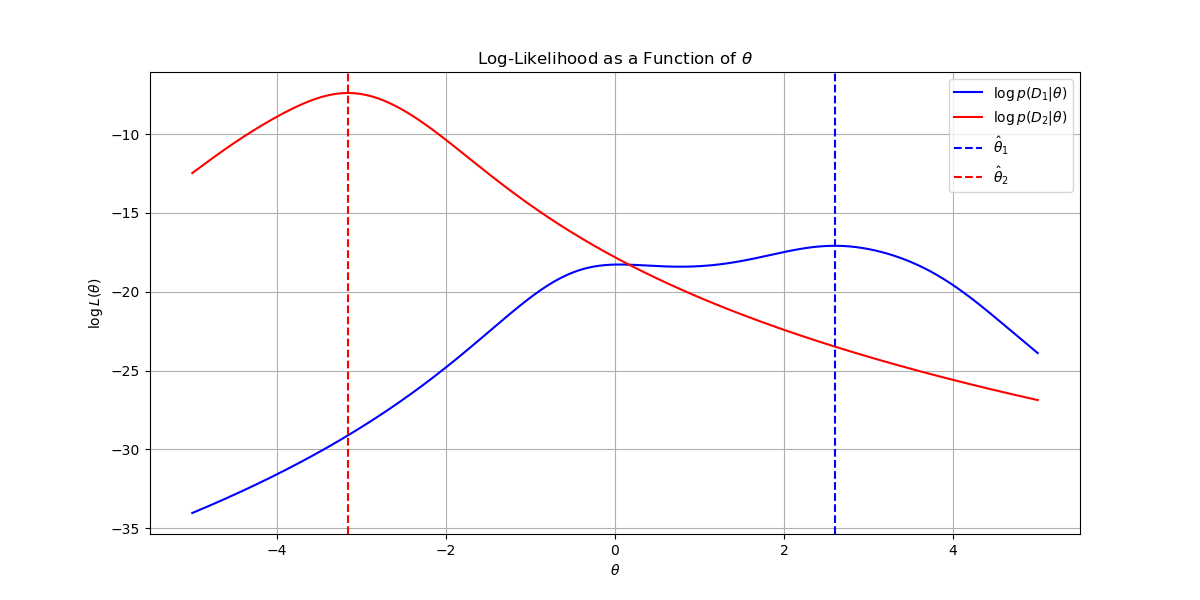
\includegraphics[width=1\linewidth]{assets/A1.png}
    \caption{Visualizing Optimal $\theta$ Values}
    \label{fig:enter-label}
\end{figure}
\end{frame}

\begin{frame}
\frametitle{A2}
Now, we need to use Discriminant Function $$ g(x) = \log P(x \mid \hat{\theta}_1) - \log P(x \mid \hat{\theta}_2) + \log P(\omega_1) - \log P(\omega_2) $$ to classify our data.
\end{frame}

\begin{frame}
\frametitle{Priors Calculation}
We calculate the \textit{a priori probabilities} for each class $\omega_i$. We have a total of 12 samples:
\begin{itemize}
    \item 7 classified in $\omega_1$
    \item 5 classified in $\omega_2$
\end{itemize}
\vspace{0.5cm}
So we calculate $P(\omega_1)=7/12$ and $P(\omega_2)=5/12$ 
\end{frame}


\begin{frame}
\frametitle{Plot}
\begin{figure}
    \centering
    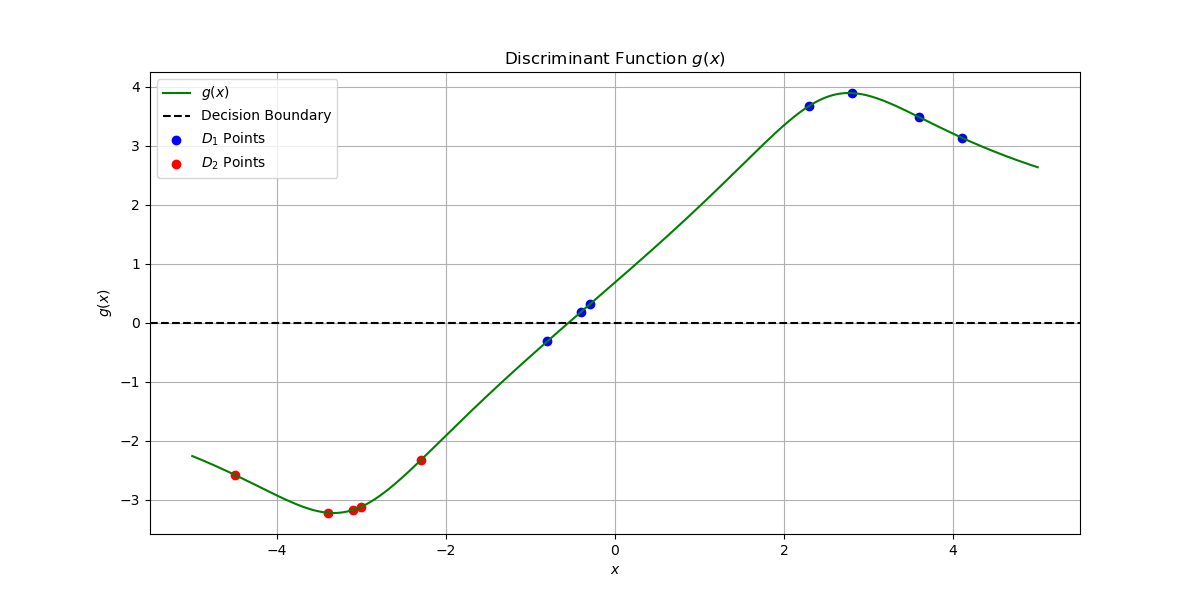
\includegraphics[width=1\linewidth]{assets/A2.png}
    \caption{Discriminant Function Visualization}
    \label{fig:enter-label}
\end{figure}
\end{frame}

\begin{frame}
\frametitle{Observations}
\begin{itemize}
    \item Most of the $D1$ points are classified correctly, as $g(x) > 0$.
    \item All of the $D2$ points are classified correctly, as $g(x) < 0$.
\end{itemize}
\vspace{1cm}
\textbf{Decision Rule:} The decision boundary is at $g(x) = 0$. For any $x$:
\begin{itemize}
    \item If $g(x) > 0$, classify $x$ as $ω1$ (no stress).
    \item If $g(x) < 0$, classify $x$ as $ω2$ (stress).
\end{itemize}
\end{frame}

\begin{frame}
\frametitle{Conclusion}
The classification rule leads to some misclassifications. While the decision rule works well for most of the data (11/12, 92\%), there are always some trade-offs in classification accuracy. Achieving perfect classification is sometimes not feasible or desirable.

\begin{itemize}
    \item Attempting to perfectly classify all points might lead to \textbf{overfitting}. A model that fits all training data perfectly may not generalize well to unseen data.
    \item The data may inherently contain some ambiguous or \textbf{overlapping} cases that no model can perfectly classify, especially if the two classes are not linearly separable.
\end{itemize}

\end{frame}

% PART B%

\begin{frame}
\frametitle{Part B}
In this part our task is to implement a new classifier for the previous problem, this time using Bayesian Estimation to estimate parameter $\theta$. 
\end{frame}


\begin{frame}
\frametitle{Data}

To perform our analysis we use the following data:
\begin{itemize}
    \item The Probability Density Functions (PDF)$$ p(\theta) = \frac{1}{10\pi \left( 1 + \left(\frac{\theta}{10}\right)^2 \right)}, \:\:\: p(x \mid \theta) = \frac{\pi}{1 + (x - \theta)^2} $$
    \item Training Samples $D_1$ and $D_2$ for both classes ($\omega_1$, $\omega_2$)
    \item A Discriminant Function $$ h(x) = \log P(x \mid D_1) - \log P(x \mid D_2) + \log P(\omega_1) - \log P(\omega_2) $$
\end{itemize}
\end{frame}

\begin{frame}
\frametitle{B1}
In this part, our goal is to calculate the a posteriori probability of $\theta$,
$$
p(\theta \mid D) = \frac{p(D \mid \theta) \cdot p(\theta)}{\int_{-\infty}^{\infty} p(D \mid \theta) \cdot p(\theta) \, d\theta}
$$
\end{frame}

\begin{frame}
\frametitle{$\theta$ Candidates}
\begin{itemize}
    \item In Part A, the dataset values were relatively small ([-4.5, 4.1]). Using a range of [-5, 5] was a practical choice because it encompassed the likely $\theta$ values where the likelihood peaks.
    \item In Part B, the prior distribution has a broader support ($(\theta / 10)$ in the denominator suggests a wider possible range). To ensure the posterior distribution adequately integrates both the likelihood and the prior, we expanded the range to [-10, 10].
\end{itemize}

\end{frame}

\begin{frame}
\frametitle{Plot}
\begin{figure}
    \centering
    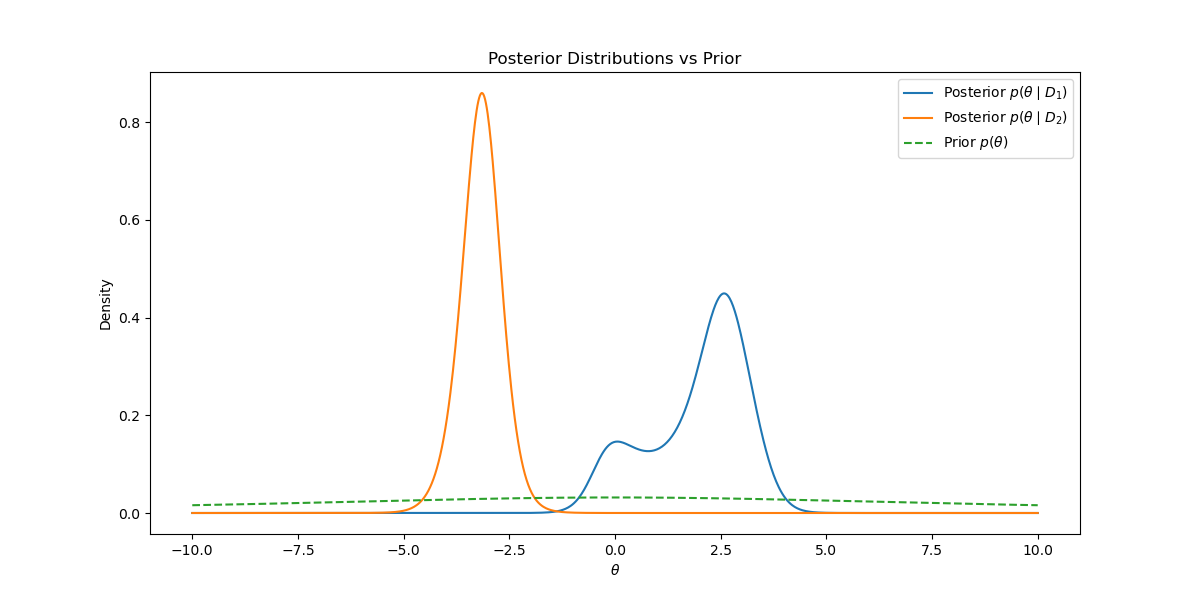
\includegraphics[width=1\linewidth]{assets/B1.png}
    \caption{$P(\theta \mid D_1)$, $P(\theta \mid D_2)$ and $P(\theta)$}
    \label{fig:enter-label}
\end{figure}
\end{frame}

\begin{frame}
\frametitle{Observations}
\begin{itemize}
    \item The prior distribution $p(\theta)$ is flat and spread out over the range of $\theta$ values. It shows minimal preference for any specific $\theta$, reflecting the prior belief before observing the data.
    \item The posteriors are much more concentrated than the prior, reflecting how the observed data updates the prior belief and provides more precise estimates of $p(\theta)$.
    \item The location of the peaks in the posteriors ($p(\theta \mid D_1)$ near 2 and $p(\theta \mid D_2)$ near -3) shows the influence of the datasets $D_1$ and $D_2$, respectively.
\end{itemize}
\end{frame}

\begin{frame}
\frametitle{B2}
We declare posterior predictive distribution $p(x \mid D)$ like so:
$$
p(x \mid D) = \int p(x \mid \theta) p(\theta \mid D) d\theta
$$

Then we declare the discriminant function $h(x)$:
$$
h(x) = \log P(x \mid D_1) - \log P(x \mid D_2) + \log P(\omega_1) - \log P(\omega_2)
$$
\end{frame}

\begin{frame}
\frametitle{Plot}
\begin{figure}
    \centering
    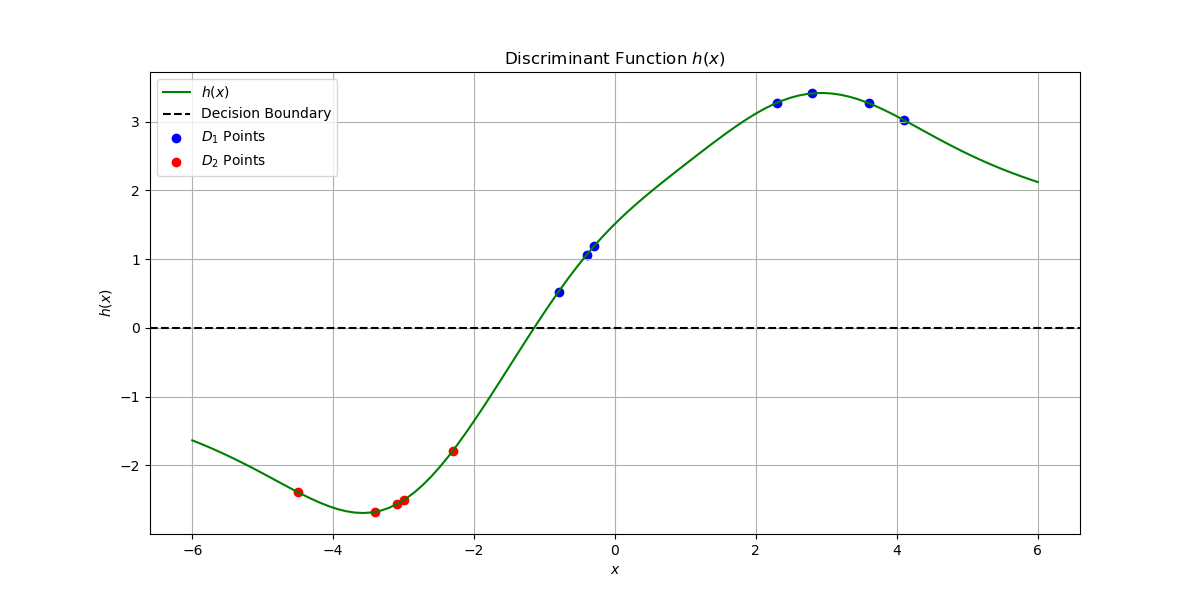
\includegraphics[width=1\linewidth]{assets/B2.png}
    \caption{Discriminant Function Visualization}
    \label{fig:enter-label}
\end{figure}
\end{frame}

\begin{frame}
\frametitle{Observations}
\begin{itemize}
    \item All of the $D1$ points are classified correctly, as $h(x) > 0$.
    \item All of the $D2$ points are classified correctly, as $h(x) < 0$.
\end{itemize}
\vspace{1cm}
\textbf{Decision Rule:} The decision boundary is at $h(x) = 0$. For any $x$:
\begin{itemize}
    \item If $h(x) > 0$, classify $x$ as $ω1$ (no stress).
    \item If $h(x) < 0$, classify $x$ as $ω2$ (stress).
\end{itemize}
\end{frame}

\begin{frame}
\frametitle{Maximum Likelihood Estimation vs Bayesian Estimation}

\textbf{Part A:}
\begin{itemize}
    \item Estimates a single value for $\theta$ ($\hat{\theta}_1$ and $\hat{\theta}_2$) that maximizes the likelihood for each class.
    \item The decision boundary is determined by the log-likelihood and prior probabilities.
\end{itemize}



\textbf{Part B:}
\begin{itemize}
    \item Considers the entire distribution of $\theta$ given the data (the posterior distribution) to make predictions.
    \item The decision boundary is determined by the posterior predictive distribution,  which integrates over all possible values of $\theta$ weighted by their posterior probabilities.
\end{itemize}

We attribute the better performance of BE to the fact that we have prior knowledge about the parameter $\theta$, in means of $p(\theta)$.

\end{frame}

% PART C%

\begin{frame}
\frametitle{Part C}
In this part, our study focuses on the classification of three Iris species: Iris setosa, Iris versicolor, and Iris virginica (i.e. three \textit{classes}).
\begin{itemize}
    \item Using the \textbf{sklearn} library, we analyze a dataset of 150 measurements (50 per species).
    \item Only the first two features (sepal length and width) are used.
    \item A DecisionTreeClassifier is implemented to classify 50\% of randomly selected samples after training the model on the remaining 50\%.
\end{itemize}
   
\end{frame}

\begin{frame}
\frametitle{C1.1}
Our goal is to find the optimal depth with respect to \textit{accuracy}. To do so, we iterate in a range of possible depths (1,10), where the optimal depth should lie. We chose this particular range to avoid overfitting. 
\begin{itemize}
    \item Deep descision trees generally lead to overfitting -they tend to capture overly specific patterns that do not generalize well.
    \item This is especially true in our case, where the dataset is relatively small (150 samples).
\end{itemize}

\end{frame}

\begin{frame}
\frametitle{Plot}
We create the \textbf{Decision Tree} that yields the best \textit{accuracy}. As shown in the plot, the optimal \textbf{depth} is 3 with \textbf{accurracy} 0.79.
\begin{figure}
    \centering
    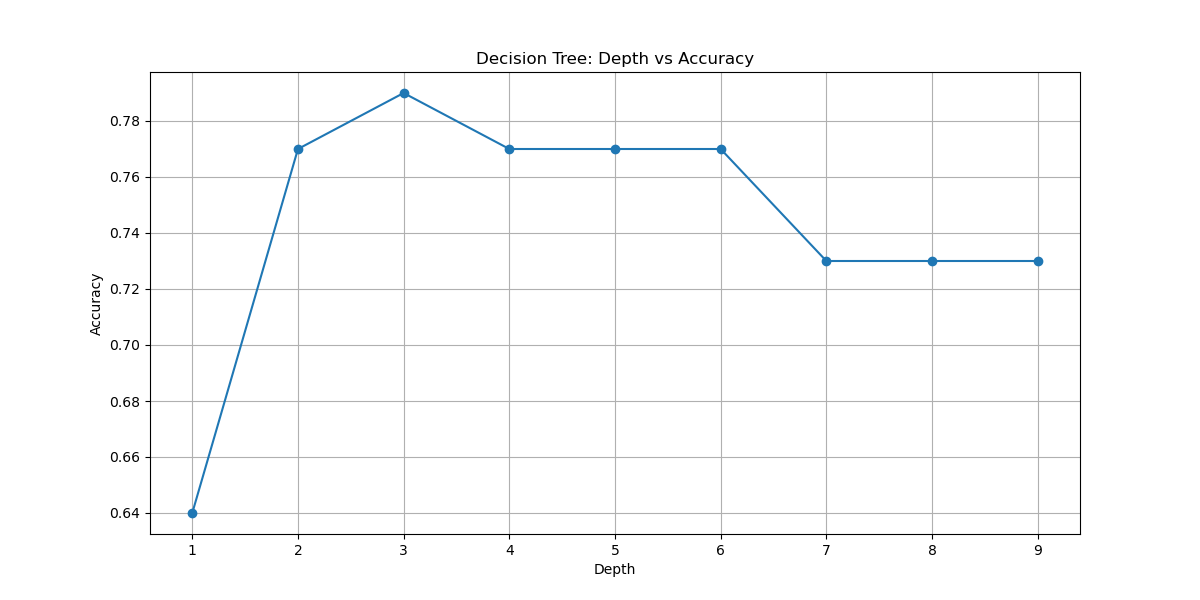
\includegraphics[width=1\linewidth]{assets/C1.1.png}
    \caption{Optimal Depth}
    \label{fig:enter-label}
\end{figure}
\end{frame}

\begin{frame}
\frametitle{C1.2}
\begin{figure}
    \centering
    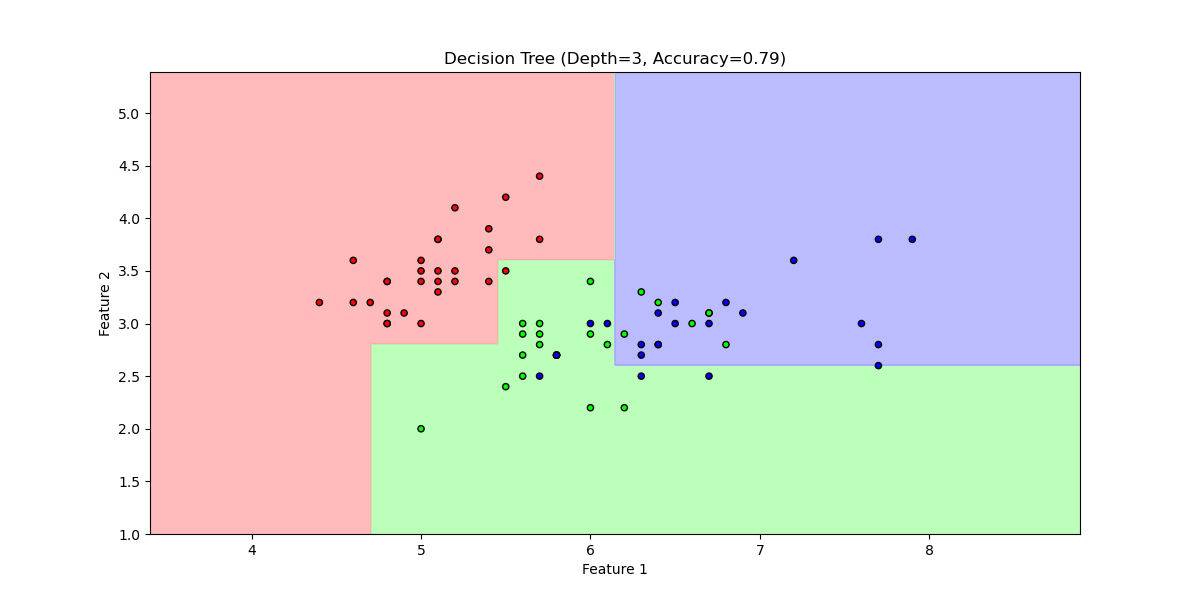
\includegraphics[width=1\linewidth]{assets/C1.2.png}
    \caption{Classification}
    \label{fig:enter-label}
\end{figure}
\end{frame}

\begin{frame}
\frametitle{C2.1}
In this task, we extend our classification of the three Iris species using a \textbf{Random Forest} classifier with \textit{100 decision trees}. 
\begin{itemize}
    \item From the training set used previously (set A, 50\% of the dataset), we create 100 training sets, each consisting of $\gamma = 50\%$ of set A, using the \textbf{bootstrap} method.
    \item Each decision tree is trained on its respective bootstrap set with a fixed maximum depth.
    \item The test set from the previous task is reused to evaluate the performance of the Random Forest classifier.
\end{itemize}
\end{frame}

\begin{frame}
\frametitle{Optimal Depth}
Our goal is yet again to find the optimal depth with respect to \textit{accuracy}. To do so, we iterate in a range of possible depths (1,10), where the optimal depth should lie.
\end{frame}

\begin{frame}
\frametitle{Plot}
We create the \textbf{Random Forest} that yields the best \textit{accuracy}. As shown in the plot, the optimal \textbf{depth} is 2 with \textbf{accurracy} 0.83.
\begin{figure}
    \centering
    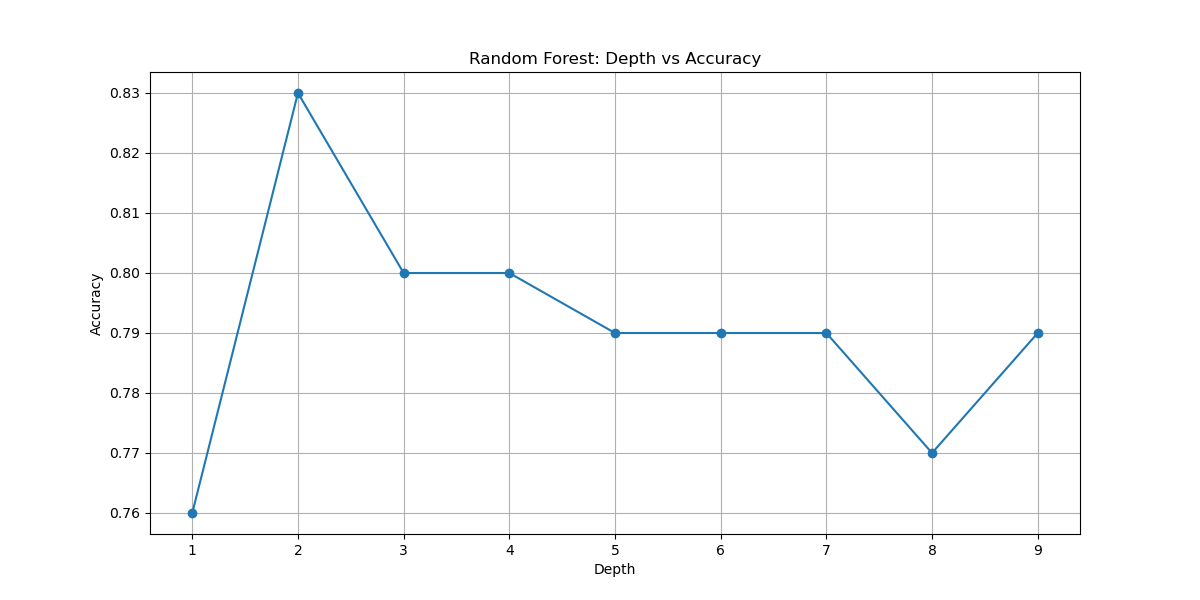
\includegraphics[width=1\linewidth]{assets/C2.1.png}
    \caption{Optimal Depth}
    \label{fig:enter-label}
\end{figure}
\end{frame}

\begin{frame}
\frametitle{C2.2}
\begin{figure}
    \centering
    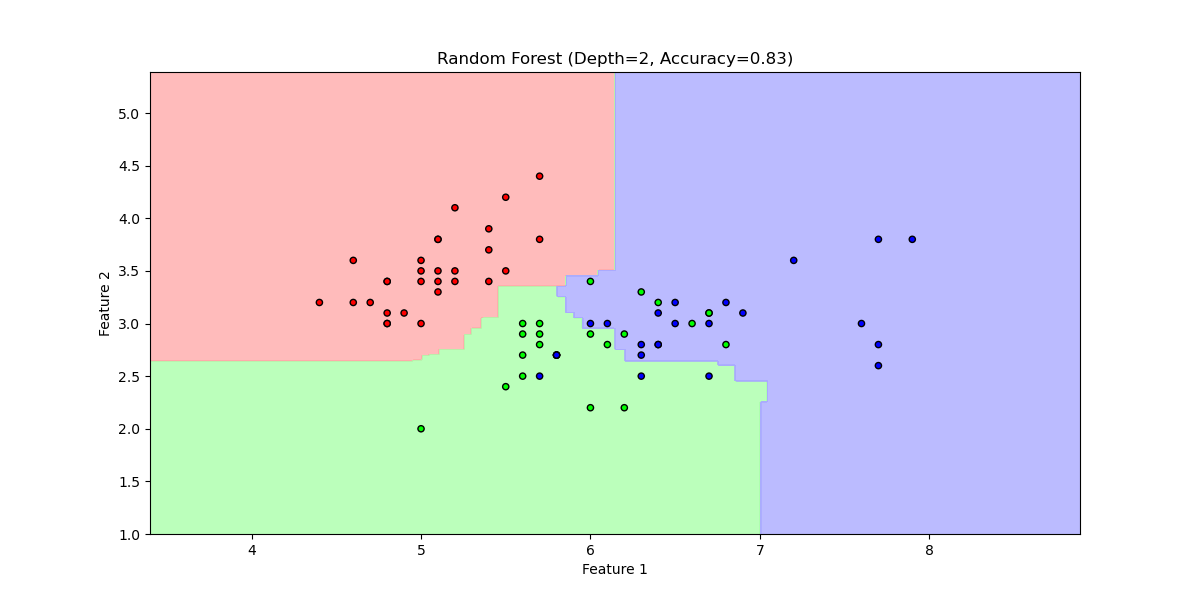
\includegraphics[width=1\linewidth]{assets/C2.2.png}
    \caption{Enter Caption}
    \label{fig:enter-label}
\end{figure}
\end{frame}

\begin{frame}
\frametitle{C2.3}

We calculate the \textit{accuracy} achieved for different values of $\gamma$ on its respective best depth. Essentially, we keep the \textit{best} result we can get for each $\gamma$, as an example. 

\begin{itemize}
    \item For lower values of $\gamma$ (0.1, 0.2, 0.3), the best accuracy varies between 0.80 and 0.81, with slight improvements as gamma increases. 
    \item For higher values (0.4 and above), the accuracy stabilizes at around 0.83, indicating diminishing returns in performance improvement with increasing gamma. 
    \item The best depth remains practically constant and equal to 2 for almost every $\gamma$.
\end{itemize}

\end{frame}

\begin{frame}
\frametitle{$\gamma$ Influence}
\begin{itemize}
    \item Generally, small $\gamma$ leads to \textbf{higher bias}, because each bootstrap set contains less information about the entire dataset.
    \item On the other hand, for bigger values of $\gamma$ the diversity among bootstrap sets decreases, which can reduce the ensemble's effectiveness at reducing variance.
\end{itemize}
\vspace{0.5cm}
In conclusion, increasing $\gamma$ up to 0.4 seems to benefit our algorithm, but further increasing it does not have any effect on \textit{accuracy} or the best depth for the Random Forest.
\end{frame}

% PART D%

\begin{frame}
\frametitle{PART D}
In this part, our task is to use datasetTV.csv to train a classifier of our choosing, which will be tested with datasetTest.csv. We are dealing with a classification problem with the following characteristics:
\begin{itemize}
    \item 5-class classification problem
    \item 8743 training samples
    \item 224 features
\end{itemize}
\end{frame}

\begin{frame}
\frametitle{Data Visualization}
Our first move was to attempt to visualize our data. Since our data lie in high-dimensional space, it would be impossible to illustrate it. So, we performed PCA (dimensionality reduction) and projected the dataset in the 3D space, in an attempt to draw conclusions from the visual. 
\end{frame}

\begin{frame}
\frametitle{Data Visualization}
\begin{figure}
    \centering
    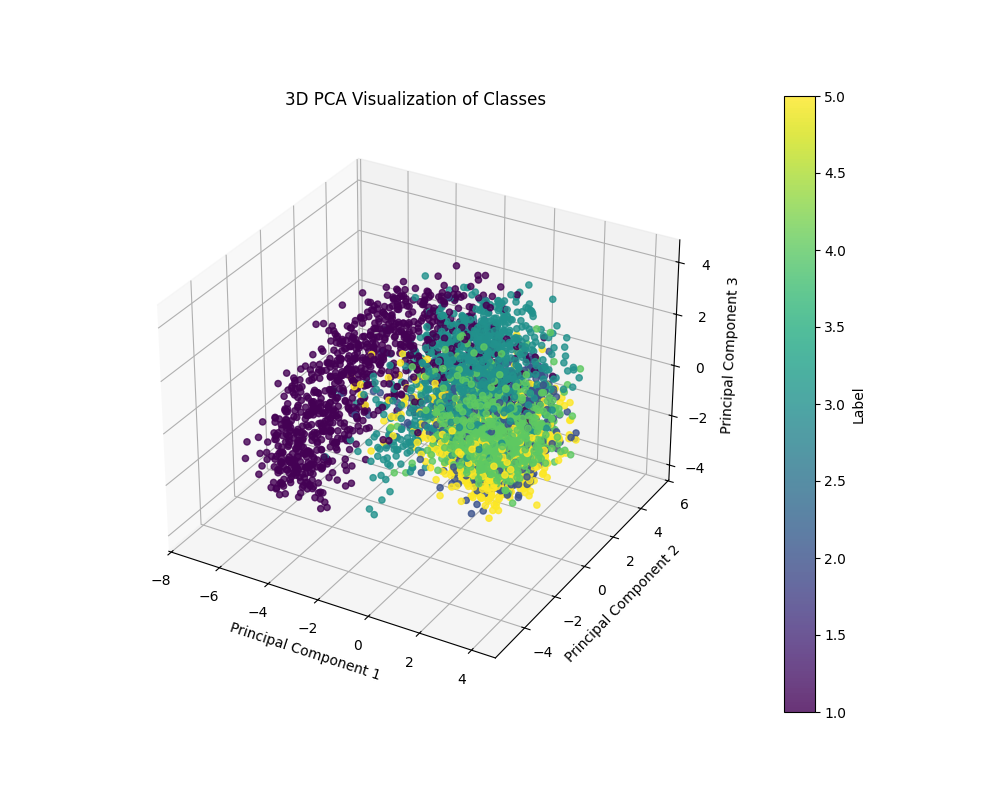
\includegraphics[width=1\linewidth]{assets/datasetTV.png}
    \caption{Enter Caption}
    \label{fig:enter-label}
\end{figure}
\end{frame}

\begin{frame}
\frametitle{Kernel Search}
The visual representation is not of great help, but is a starting point for our analysis. 

Our next attempt was to find a kernel in hopes that the dataset is \textbf{linear separable}. That would make approaches like:
\begin{itemize}
    \item SVM
    \item Logistic Regression
    \item Naive Bayes
\end{itemize}
suitable for our classifier.
\end{frame}

\begin{frame}
\frametitle{Silhouette Score}
In order to check whether the transformed kernel data is linearly separable, we will use the \textbf{silhouette score} as a metric. 
The silhouette score quantifies how well a data point fits into its class and ranges from -1 to 1:
\begin{itemize}
    \item  1: Perfectly matched to its class (linearly separable classes).
    \item  0: On the boundary between classes.
    \item -1: Misclassified, closer to another class (non-linearly separable classes).
\end{itemize}
\end{frame}

\begin{frame}
\frametitle{Results}
The silhouette score for the original dataset is 0.01.
\vspace{0.5cm}
\begin{table}[ht]
\centering
\begin{adjustbox}{max width=\textwidth}
\begin{tabular}{@{}lccccc@{}}
\toprule
\textbf{Kernel} & \textbf{$\gamma$: 0.001} & \textbf{$\gamma$: 0.01} & \textbf{$\gamma$: 0.1} & \textbf{$\gamma$: 1} & \textbf{$\gamma$: 10} \\ \midrule
\textbf{rbf}     & 0.03                 & 0.03                & -0.37              & -0.03            & -0.03            \\
\textbf{poly}    & 0.03                 & -0.00               & -0.07              & -0.09            & -0.09            \\
\textbf{sigmoid} & 0.03                 & 0.03                & 0.03               & 0.03             & 0.04             \\
\textbf{cosine}  & 0.04                 & 0.04                & 0.04               & 0.04             & 0.04             \\ \bottomrule
\end{tabular}
\end{adjustbox}
\caption{Silhouette Scores for Different Kernels and $\gamma$ Values}
\label{tab:silhouette_scores}
\end{table}
\end{frame}

\begin{frame}
\frametitle{Conclusions}
As we can see from the above results, the silhouette scores of the original and transformed data range from -0.37 to 0.04. This indicates that our data are not linearly separable.
\end{frame}

\begin{frame}
\frametitle{Testing Multiple Classifiers}
To verify our hypothesis about the poor performance of linear approaches, we conducted a general search for the optimal classifier, using some default and generic parameters so that we get an idea of what performs best for our dataset.
\end{frame}

\begin{frame}[fragile]
\frametitle{Models}
These are the models we tested with their respective parameters: \vspace{0.5cm}
\lstset{style=PythonStyle}
\begin{lstlisting}
"Decision Tree": DecisionTreeClassifier(random_state=42),
    
"KNN(5NN)": KNeighborsClassifier(n_neighbors=5),
"Naive Bayes": GaussianNB(),

"Logistic Regression": LogisticRegression(max_iter=300, random_state=42),
"Perceptron": Perceptron(max_iter=300, random_state=42),
"Least Squares": RidgeClassifier(),

"SVM": SVC(kernel='linear', random_state=42),

"Neural Network": MLPClassifier(
    hidden_layer_sizes=(100,), max_iter=300, random_state=42),

"Random Forest": RandomForestClassifier(n_estimators=100, random_state=42),

"AdaBoost": AdaBoostClassifier(n_estimators=100, random_state=42)
\end{lstlisting}
\end{frame}

\begin{frame}
\frametitle{Cross-Validation Accuracy}
To test the performance of every model we used \textbf{5-fold cross validation}:
\begin{itemize}
    \item The dataset is randomly divided into 5 equal parts (or folds). Each fold is used once as a test set while, the other 4 are used for training.
    \item For each iteration, the model is trained on the training set and its accuracy is evaluated on the test set.
    \item Once all 5 iterations are complete, calculate the average of the accuracies from all folds to get the cross-validation accuracy.
\end{itemize}
\end{frame}

\begin{frame}
\frametitle{5-Fold Cross-Validation}
\begin{figure}
    \centering
    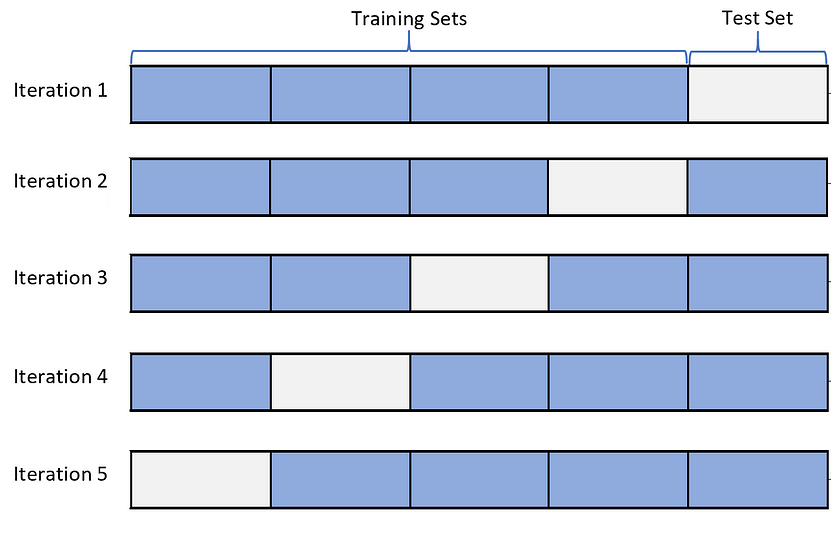
\includegraphics[width=0.8\linewidth]{assets/cross-validation.png}
    \caption{5-fold Cross Validation}
    \label{fig:enter-label}
\end{figure}
\end{frame}

\begin{frame}
\frametitle{Results}

\begin{table}[ht]
\centering
\label{tab:cross_validation_accuracy}
\begin{adjustbox}{max width=\textwidth}
\begin{tabular}{@{}lc@{}}
\toprule
\textbf{Model} & \textbf{Cross-Validation Accuracy} \\ \midrule
Decision Tree      & 0.62 \\
KNN(5NN)           & 0.81 \\
Naive Bayes        & 0.70 \\
Logistic Regression & 0.77 \\
Perceptron         & 0.69 \\
Least Squares      & 0.75 \\
SVM                & 0.76 \\
Neural Network     & 0.83 \\
Random Forest      & 0.80 \\
AdaBoost           & 0.65 \\ \bottomrule
\end{tabular}
\end{adjustbox}
\caption{Cross-Validation Accuracy for Different Models}
\end{table}
\end{frame}

\begin{frame}
\frametitle{Candidates}
Out of all the classifiers we tested, we separated the
\begin{itemize}
    \item k-Nearest Neighbors
    \item Random Forest 
    \item Neural Network
\end{itemize} 
classifiers as the best scoring in terms of accuracy. \vspace{0.5cm}

These results align with our hypothesis that our data are not linear separable. Our goal now is to tune the parameters of said classifiers, in order to maximize the cross-validation accuracy and decide on our final model. To do so we performed a grid search for each one of them.
\end{frame}

\begin{frame}[fragile]
\frametitle{KNN Tuning}
\lstset{style=PythonStyle}
\begin{lstlisting}
param_grid = {
    'n_neighbors': [3, 5, 7, 9, 11],
    'weights': ['uniform', 'distance'],
    'metric': ['euclidean', 'manhattan', 'minkowski', 'cosine'],
    'p': [1, 2],
    'algorithm': ['auto', 'ball_tree', 'kd_tree', 'brute']
}
\end{lstlisting}
Best cross-validation accuracy: \textbf{0.83} \\
Best parameters found: 
\begin{itemize}
    \item 'n\_neighbors': 9
    \item 'weights': 'distance'
    \item 'metric': 'cosine'
    \item 'p': 1
    \item 'algorithm': 'auto'
\end{itemize}
\end{frame}

\begin{frame}[fragile]
\frametitle{RF Tuning}
\lstset{style=PythonStyle}
\begin{lstlisting}
param_grid = {
    'n_estimators': [200, 300, 400, 500],
    'criterion': ['gini', 'entropy'],
    'max_depth': [10, 20, 50, None],
    'min_samples_split': [5, 10, 20],
    'min_samples_leaf': [2, 5, 10],
    'class_weight': ['balanced', None],
    'max_features': ['auto', 'sqrt', 'log2'],
    'bootstrap': [True, False]
}
\end{lstlisting}
Best cross-validation accuracy: \textbf{0.83} \\
Best parameters found: 
\begin{columns}
    \begin{column}{0.5\textwidth}
        \begin{itemize}
            \item \texttt{'n\_estimators'}: 500
            \item \texttt{'criterion'}: 'entropy'
            \item \texttt{'max\_depth'}: 20
            \item \texttt{'min\_samples\_split'}: 5
        \end{itemize}
    \end{column}
    \begin{column}{0.5\textwidth}
        \begin{itemize}
            \item \texttt{'min\_samples\_leaf'}: 2
            \item \texttt{'algorithm'}: 'auto'
            \item \texttt{'class\_weight'}: 'balanced'
            \item \texttt{'max\_features'}: 'sqrt'
            \item \texttt{'bootstrap'}: False
        \end{itemize}
    \end{column}
\end{columns}

\end{frame}

\begin{frame}[fragile]
\frametitle{NN Tuning}
\lstset{style=PythonStyle}
\begin{lstlisting}
param_grid = {
    'hidden_layer_sizes': [(50,), (100,), (200,), (100, 50), (100, 100)],
    'activation': ['relu', 'tanh'],
    'solver': ['adam', 'sgd', 'lbfgs'],
    'alpha': [0.0001, 0.001, 0.01],
    'learning_rate': ['constant', 'adaptive'],
    'learning_rate_init': [0.001, 0.01, 0.0001],
    'early_stopping': [True, False],
    'max_iter': [200, 300, 500]
}
\end{lstlisting}
Best cross-validation accuracy: \textbf{0.84} \\
Best parameters found:
\begin{columns}
    \begin{column}{0.45\textwidth}
        \begin{itemize}
            \item \texttt{'hidden\_layer\_sizes'}: (200,)
            \item \texttt{'activation'}: 'relu'
            \item \texttt{'solver'}: 'adam'
            \item \texttt{'alpha'}: 0.0001
        \end{itemize}
    \end{column}
    \begin{column}{0.55\textwidth}
        \begin{itemize}
            \item \texttt{'learning\_rate'}: 'constant'
            \item \texttt{'learning\_rate\_init'}: 0.01
            \item \texttt{'early\_stopping'}: False
            \item \texttt{'max\_iter'}: 200
        \end{itemize}
    \end{column}
\end{columns}
\end{frame}

\begin{frame}
\frametitle{Optimal Model}
As we can observe, the model that achieves the best cross-validation accuracy for the training set is a Neural Network with the following characteristics:
\vspace{0.5cm}
\begin{itemize}
    \item One hidden layer with 200 neurons
    \item ReLU activation function\[\text{ReLU}(x) = \max(0, x)\]
    \item Adam optimizer for weight updates
    \item Constant learning rate with an initial value of $\eta = 0.01$
\end{itemize}
\end{frame}

\begin{frame}
\frametitle{Data Scaling}
Although, before fitting the model to our data, we must preprocess it. First, we will \textbf{scale} the data, as this step is essential for models like neural networks.
\vspace{0.5cm}

Scaling improves the convergence of gradient descent and ensures that features with larger numerical ranges do not dominate the learning process.

\end{frame}

\begin{frame}
\frametitle{Feature Selection}
Moreover, our data lies in a high-dimensional space (224 dimensions), so we decided to use \textbf{feature selection}. Specifically, we used a correlation-based technique to discard features with low correlation to the label, as these are unlikely to provide meaningful information for the classification task. Using feature selection offers the following benefits:
\vspace{0.5cm}
\begin{itemize}
    \item Reduce noise in the data
    \item Decreases the risk of \textbf{overfitting} because the model focuses on learning the underlying patterns rather than memorizing noise
    \item Improves computational efficiency
\end{itemize}
\end{frame}

\end{document}